\index{COMMANDS@\textbf{COMMANDS}!\textbackslash pgfPTbuildcell!designing cells with}%
\hypertarget{buildcells}{To start designing} the \textit{base cell} of the Periodic Table it is necessary to keep in mind that each cell will be split into \textbf{n} rows and \textbf{k} columns.
\\ [6pt]As a running example, \textcolor{blue}{5} rows and \textcolor{red}{3} columns will be used:
\\ [6pt]\makebox[\linewidth][c]{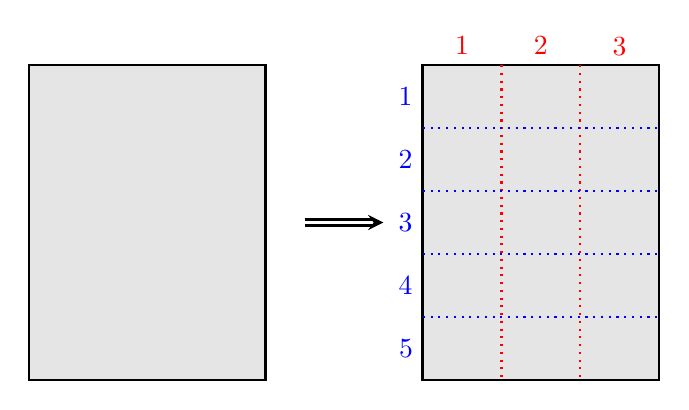
\begin{tikzpicture}
\draw[line width=1pt,fill=black!10] (0,0) rectangle ++(3,-4);
\draw[line width=1pt,double distance=1pt,-stealth] (3.5,-2) -- ++(1,0);
\draw[line width=1pt,fill=black!10] (5,0) rectangle ++(3,-4);
\foreach \x in {1,2}{\draw[dotted,line width=.8pt,red] (5cm+\x cm,0) node[above,xshift=-.5cm] {\x} -- ++(0,-4);}\node[red,above] at (7.5,0) {3};
\foreach \y in {1,...,4}{\draw[dotted,line width=.8pt,blue] (5cm,-.8*\y cm) node[left,yshift=.4cm] {\y} -- ++(3,0);}\node[blue,left] at (5,-3.6) {5};
\end{tikzpicture}}
\\ [10pt]The next task is to assign contents to the cell by typing \textit{trios} with the structure
\begin{itemize}
\item[--]\textbf{(row;column;content)}\item[--]or \textbf{(start row-end row;start column-end column;content)}\item[--]or a combination of both.
\end{itemize}
The available \textbf{contents} are: Z, name, CS, Ar, Ar*, radio, R, Rcov, Rion, Ei, eneg, eaff, O, Tmelt, TmeltC, Tboil, TboilC, eDist, eConfign, eConfignl, d, Cp, kT, ls, lsa, lsb, lsc, lsca, DiscY, DiscC and spectra.
\\ [16pt]Assigning, for instance, \green{(1;1;Z)} will show the atomic number in the first row and in the first column,
\\ [6pt]\pgfPTMcelldesign(1;1;Z)(1 to 2)(1 to 2)
\\ [6pt]while the assignment \green{(1;1-2;Z)} will show the atomic number in the first row and filling the first and second columns,
\\ [6pt]\pgfPTMcelldesign(1;1-2;Z)(1 to 2)(1 to 3)
\\ [10pt]It is also possible to start at a \textit{fraction} of a line or column. If it is intended to start a line at the middle of the first column the value used should be \green{1.5}, which means that the start value is at the half (\textit{0.5}) of the first column (\textit{1}), observing that \textit{1.5} is \textit{0.5} plus \textit{1}:
\\ [6pt]\pgfPTMcelldesign(1;1.5;Z)(1 to 2)(1.5 to 2.5)
\\ [10pt]As in the second example above it is possible to end up in a specified \textit{fraction} of a line or column:
\\ [6pt]\pgfPTMcelldesign(1;1.5-3.5;Z)(1 to 2)(1.5 to 3.5)
\\ [48pt]\tikz{\node[text width=\linewidth-.6666em,fill=green!5!white,draw=green!50!black,rounded corners=2pt] {%
\index{COMMANDS@\textbf{COMMANDS}!\textbackslash pgfPTbuildcell!row, column syntax}%
\textbf{\large The \green{row}, \green{column} \textit{syntax}}
\\ [6pt]Both lines and columns share the same syntax,  where \green{n} is any integer between 1 and the number of rows and \green{f} is the fractional part of any number between 0 and 1:
\begin{itemize}
\item[\bfseries(1)] If only the row number \green{n} is provided the \textit{content} is placed at the row \green{n} .
\item[\bfseries(2)] If the row number \green{n} is provided followed by a \green{dot} and a number \green{f}, the \textit{content} is placed at the fraction \green{f} of the row \green{n}.
\item[\bfseries(3)] If the start row \green{n}\raisebox{-1.5pt}{\small s} and the end row \green{n}\raisebox{-1.5pt}{\small e} are provided separated by a \green{dash}, \ie, \green{n}\raisebox{-1.5pt}{\small s}-\green{n}\raisebox{-1.5pt}{\small e}, the \textit{content} is placed filling all the rows from \green{n}\raisebox{-1.5pt}{\small s} to \green{n}\raisebox{-1.5pt}{\small e}.
    \\ [2pt]\textit{The \green{dot} notation described in }\textbf{(2)} \textit{can be used both on }\green{n}\raisebox{-1.5pt}{\small s} \textit{and } \green{n}\raisebox{-1.5pt}{\small e}.
\item[\bfseries(4)] All of the items above apply to columns in the same way.
\end{itemize}
};}
\subsection{\texorpdfstring{$\maltese$ The cell contents}{The cell contents}}
\makeatletter%
\setbox0=\hbox{\pgfPT@set@econfig[]{[Ar]::3d+1,4s+2}}%
\setbox1=\hbox{\pgfPT@set@econfig[]{[Ar]::4s+2,3d+1}}%
\makeatother%
\begin{itemlist}\hangindent=50pt
\item\textbf{Z} -- the atomic number of the elements.
\item\textbf{name} -- the name of the elements.
\item\textbf{CS} -- the chemical symbol of the elements.
\item\textbf{Ar} -- the relative atomic mass (atomic weight) of the elements.
\item\textbf{Ar*} --the standard relative atomic mass (standard atomic weight) of the elements.
\item\pgfPTMparbox{\textbf{radio} -- radioactivity of the elements. If the element is radioactive the figure \includegraphics[height=6.5pt]{pgfPT_radio_symbol.pdf} is placed in the cell, otherwise nothing is shown.}
\item\pgfPTMparbox{\textbf{R} -- the atomic radius of the elements. The atomic radius shown is the calculated radius and is expressed in picometers.}
\item\pgfPTMparbox{\textbf{Rcov} -- the covalent radius of the elements. The covalent radius shown is for single bonds and is expressed in picometers.}
\item\pgfPTMparbox{\textbf{Rion} -- the ionic radius of the elements. The radius shown is the effective ionic radius in picometers.}
\item\pgfPTMparbox{\textbf{Ei} -- the first ionization energy of the elements, measured in {\large$\mathsf{kJ\cdot mol^{-1}}$}. All data from rutherfordium onwards is predicted.}
\item\textbf{eneg} -- the Pauling electronegativity of the elements.
\item\pgfPTMparbox{\textbf{eaff} -- the electroaffinity (electron affinity) of the elements, measured in {\large$\mathsf{kJ\cdot mol^{-1}}$}. Estimated negative values have been replaced by zero, since the negative ions formed in these cases are always unstable (they may have lifetimes of the order of microseconds to milliseconds, and invariably autodetach after some time).}
\item\textbf{O} -- the common oxidation states of the elements.
\item\textbf{Tmelt} -- the melting point, in Kelvin, of the elements.
\item\textbf{TmeltC} -- the melting point, in degrees Celsius, of the elements.
\item\textbf{Tboil} -- the boiling point, in Kelvin, of the elements.
\item\textbf{TboilC} -- the boiling point, in degrees Celsius, of the elements.
\item\textbf{eDist} -- the electron distribution of the elements.
\item\pgfPTMparbox{\textbf{eConfign} -- the electronic configuration, in increasing n (principal quantum number), of the element, corresponding to the \textit{spectroscopic} order of orbital energies, that is, the reverse of the order in which electrons are removed from a given atom to form positive ions.}
\\ [6pt]\makebox[.1\linewidth][s]{}\begin{minipage}{.9\linewidth}\footnotesize\blue{\textit{\textbf{Note}: the short version of the electronic configuration is used, \ie, [previous noble gas]remaining electrons. For example, for scandium it is: \scalebox{2}{\usebox0}}}\end{minipage}
\item\pgfPTMparbox{\textbf{eConfignl} --  the electronic configuration, in increasing sum of n and {\large$\ell$} (azimuthal quantum number), of the element, following the order based on the Madelung rule.}
\\ [6pt]\makebox[.1\linewidth][s]{}\begin{minipage}{.9\linewidth}\footnotesize\blue{\textit{\textbf{Note}: the short version of the electronic configuration is used, \ie, [previous noble gas]remaining electrons. For example, for scandium it is: \scalebox{2}{\usebox1}}}\end{minipage}
\item\pgfPTMparbox{\textbf{d} -- the density of the elements, in the corresponding physical state, at 25{\large$\mathsf{^oC}$} and 1{\large$\mathsf{\,atm}$}.}
\item\textbf{Cp} -- the specific heat capacity of the elements in {\large$\mathsf{J\cdot mol^{-1}\cdot K^{-1}}$} at 25{\large$\mathsf{^oC}$} and 100{\large$\mathsf{\,kPa}$}.
\item\textbf{kT} -- the thermal conductivity of the elements in {\large$\mathsf{J\cdot m^{-1}\cdot K^{-1}}$} at 25{\large$\mathsf{^oC}$}.
\item\textbf{ls} -- the lattice structure of the elements at 1{\large$\mathsf{\,bar}$} and mostly at 25{\large$\mathsf{^oC}$}.
\item\textbf{lsa} -- the lattice constant {\large$a$} of the elements in picometers at 1{\large$\mathsf{\,bar}$} and mostly at 25{\large$\mathsf{^oC}$}.
\item\pgfPTMparbox{\textbf{lsb} -- the lattice constant {\large$b$} of the eligible elements in picometers at 1{\large$\mathsf{\,bar}$} and mostly at 25{\large$\mathsf{^oC}$}.}
\item\pgfPTMparbox{\textbf{lsc} -- the lattice constant {\large$c$} of the eligible elements in picometers at 1{\large$\mathsf{\,bar}$} and mostly at 25{\large$\mathsf{^oC}$}.}
\item\textbf{lsca} -- the lattice {\large$c/a$} ratio of the eligible elements at 1{\large$\mathsf{\,bar}$} and mostly at 25{\large$\mathsf{^oC}$}.
\item\textbf{DiscY} -- the discovery year of the elements.
\item\textbf{DiscC} -- the discovery country or in, a few cases, region (Middle East or Asia Minor) of the elements.
\item\pgfPTMparbox{\textbf{spectra} -- the emission spectrum of the elements. The spectrum is only shown if available. The spectra are pre-built using the package \href{https://ctan.org/pkg/pgf-spectra}{\large\textsf{pgf-spectra}}\ via the commands:}
    \\ [8pt]\makebox[10pt][s]{}\tikz{\node[text width=\linewidth-.6666em-10pt,fill=green!5!white,draw=green!50!black,rounded corners=2pt] 
    \\ \makebox[3cm][s]{}relative intensity,relative intensity threshold=.375,\textcolor{black!50}{\small\%}
    \\ \makebox[3cm][s]{}brightness=.5,charge=all,Imin=.125,gamma=1}\blue{]}%
    \\ \red{\textbackslash foreach \textbackslash SQ in \{H,He,(...),Bi,Po,Rn,Fr,(...),Es\}}\textcolor{black!50}{\small\% Z=1,2,(...),83,84,86,87,(...),99}
    \\ \makebox[1.6cm][s]{}\red{\{}\textcolor{black!50}{\small\%}
    \\ \makebox[1.6cm][s]{}\blue{\textbackslash pgfspectra[}\red{element=\textbackslash SQ}\blue{]}\textcolor{black!50}{\small\%}
    \\ \makebox[1.6cm][s]{}\red{\}}\textcolor{black!50}{\small\%}};}
\end{itemlist}
\vfill%
\subsection{\texorpdfstring{$\maltese$ Built-in cell styles}{Built-in cell styles}}
There is a set of \textit{built-in} cell styles that could be used for the described purposes:
\index{BUILT-IN@\textbf{BUILT-IN}!
cell styles}%
\vspace{12pt}%
\begin{itemlist}
\item\pdfbookmark[3]{pgfPT2lang}{pgfPT2lang}\pgfPTMparbox{\textbf{pgfPT2lang} --  a cell layout to use with the name in two languages.}
\\ [6pt]\pgfPTpreviewcellstyle[1.6]{pgfPT2lang}\\
\item\pdfbookmark[3]{pgfPT3lang}{pgfPT3lang}\pgfPTMparbox{\textbf{pgfPT3lang} --  a cell layout to use with the name in three languages.}
\\ [6pt]\pgfPTpreviewcellstyle[1.6]{pgfPT3lang}\\
\item\pdfbookmark[3]{pgfPTR}{pgfPTR}\pgfPTMparbox{\textbf{pgfPTR} -- a cell layout to display the atomic radius and its periodic variations (if of course the \red{show periodic variations} key is set to true).}
\\ [6pt]\pgfPTpreviewcellstyle[1.6]{pgfPTR}
\newpage%
\item\pdfbookmark[3]{pgfPTEi}{pgfPTEi}\pgfPTMparbox{\textbf{pgfPTEi} -- a cell layout to display the first ionization energy and its periodic variations (if of course the \red{show periodic variations} key is set to true).}
\\ [6pt]\pgfPTpreviewcellstyle[1.6]{pgfPTEi}\\
\item\pdfbookmark[3]{pgfPTeaff}{pgfPTeaff}\pgfPTMparbox{\textbf{pgfPTeaff} -- a cell layout to display the electron affinity and its periodic variations (if of course the \red{show periodic variations} key is set to true).}
\\ [6pt]\pgfPTpreviewcellstyle[1.6]{pgfPTeaff}\\
\item\pdfbookmark[3]{pgfPTREi}{pgfPTREi}\pgfPTMparbox{\textbf{pgfPTREi} -- a cell layout to display the atomic radius and first ionization energy and their periodic variations (if of course the \red{show periodic variations} key is set to true).}
\\ [6pt]\pgfPTpreviewcellstyle[1.6]{pgfPTREi}\\
\item\pdfbookmark[3]{pgfPTls}{pgfPTls}\pgfPTMparbox{\textbf{pgfPTls} -- a cell layout to display the lattice system.}
\\ [6pt]\pgfPTpreviewcellstyle[1.6]{pgfPTls}
\newpage%
\item\pdfbookmark[3]{pgfPTdisc}{pgfPTdisc}\pgfPTMparbox{\textbf{pgfPTdisc} -- a cell layout to display the discovery country and discovery year.}
\\ [6pt]\pgfPTpreviewcellstyle[1.6]{pgfPTdisc}\\
\end{itemlist}
\endinput
